\documentclass{ctuthesis}
\usepackage{mathtools}
\usepackage{subfig}
\usepackage{xcolor}
\usepackage{listings}
\usepackage{xparse}


\lstset{language=C,keywordstyle={\bfseries \color{blue}}}


\ctusetup{
	xdoctype = B,
	xfaculty = F3,
	mainlanguage = english,
	secondlanguage = czech,
	title-english = {Planning routes for recreational cycling},
	title-czech = {Plánování tras pro rekreační cyklistiku},
	department-english = {Department of Computer Science},
	author = {Miroslav Matocha},
	supervisor = {doc. Ing. Michal Jakob, Ph.D.},
	supervisor-address = {Fakulta elektrotechnická, Resslova 307/9, Praha},
	month = 6,
	year = 2019,
	day = 6,
	keywords-english = {route planning, cycles},
	keywords-czech = {plánování cest, cykly}
}

\ctuprocess
\begin{abstract-english}
	
\end{abstract-english}
\begin{abstract-czech}
	
\end{abstract-czech}


% Acknowledgements / Podekovani
\begin{thanks}
	Thanks to CTU for beeing so great \emph{alma mater}.
\end{thanks}

% Declaration / Prohlaseni
\begin{declaration}
	I declare that I wrote this paper by myself and that I mentioned all used literature in bibliography section.
	
	In Prague, \ctufield{day}.~\monthinlanguage{title}~\ctufield{year}
\end{declaration}

\NewDocumentCommand{\codeword}{v}{
\texttt{\textcolor{blue}{#1}}
}

\begin{document}
\maketitle
\chapter{Introduction}
People are nowadays pretty used to planning and navigating their trips with the help of various map applications, thanks to the rapid spread of GPS technology especially in mobile phones in the past years. The problem of getting optimal route from A to B according to single value evaluation of the road network graph is, thanks to this intensive usage and various achievments in this field, practically completely solved. These are also the reason why people are starting to get into other areas of planning trips and trying to apply obtained knowledge to wider set of problems. This for example includes multicriterial planning, or planning in dynamic networks. \par

In this paper I am focused on breaking down the problem of using algorithmically planned routes for recreational activities. This is specific for several reasons. For example people which are interested in using generated routes for jogging or cycling are just rarely interested in specific route in terms of visited points or area. Instead they prefer to get several suggestions based on total cost of route instead (in terms of total length or travel time). Another property of these routes should be optimization of total or mean plesantness. This is whole another aspect of the problem as pleasantness of the edge can mean anything from type of communication through interesting surroundings of the edge to the proximity to some points of interest. It can even mix several criterions and can be personalized to specific user. The next important thing for our application is to put some consideration into the shape of the planned route also. Let me explain. The most used case for this type of planning algorithm would be (as we know from various fitness applications) getting suggestions for some nice cycling trip that starts and ends right at your home and therefore forms a cycle. But imagine living alongside long road with the highest pleaseantness around. All optimal trips in term of trip weight would be planned alongside this road. We could easily see, that this is not the result we crave for. So we have to take the shape of the trip or its visited areas into the account when planning. We aim for as round and "smooth" trip as possible but we also have to combine this with mentioned pleasseantness. \par



I belive this is enough of introduction into the problematics. In the next chapters I will try to  analyze simillar work which was done in this field in the past. Then I take apart the individual parts of the problem in attempt to formalize it properlly. Finally I introduce two methods for generating some feasible solution to this problem together with their implementations which I have created. In the last section I am going to present and interpret the testing results when comparing these two methods by various criteria.



\chapter{Related work}

One of the most general papers laying down the theory needed for solution of this problem is problem of finding the minimum mean cycle in the graph. \cite{karp} This problem is defined as finding the circle in the graph whose sum of weights through all edges divided by count of edges is minimal. Karp provides formula that yields the minimum mean of the mentioned cycle with linear complexity. Moreover it shows a simple technique to obtain not only this number but also the actual cycle from the same calculation. Although helpful, this technique ignores the length or cost constraint which is crucial to our application.\par

The next paper from Gemsa \cite{jogging} introduces several techniques to generate feasible enclosed jogging routes. First it focuses on solving the problem through dual graph which consists of faces from original graph as nodes connected by edges only if the coresponding faces share one or more of theirs outlining edges in original graph. This of course requires simple preprocessing step based on right hand deep searches in original graph. After the dual graph is obtained the BFS is run over it starting from node which corresponds to the face incident with starting node. The result of BFS is enclosed jogging route in every iteration. This jogging route is constructed from the border edges of the search tree. This holds as far as two conditions are met. To get simple cycle from border edges the search tree has to be connected. And it has to exclude at least one face incident with starting node to ensure that starting node is part of that border. Both of the properties are constantly checked for during algorithm execution. BFS is finnished as soon as the length criterium is fullfilled. Gemsa introduces one more technique to optimize badness of the jogging route. Another metric influencing the execution of the BFS is added to the mix. This metric consists of force field which assigns a vector to every point in the plannar graph. This vector is counted from simple formula using individual face badness normalized by distance to the power of two. This formula is iterated and summed over all faces in the graph. BFS is then edited in manner of expanding the face which center has the biggest force in the direction of extension. They call this solution Greedy Faces.\par

Second approach which is introduced is called Partial Shortest Paths. This approach is working with computing triangles(or rectangles) which fulfill the length criterion and have starting node as one of its vertices. It does so by computing the search tree of acceptable candidates from starting node. This search tree is called ring and it is constrained by third of the length of the route. From these results one via node is selected and its ring is computed with the same parameters. Then we can take the intersection area and pick the third point from there. Last step is to compute shortest paths between all three mentioned nodes, this yields one of feasible cycles. All the results from this proccess are then filtered to provide just the ones with best mean badness. \par
This approach provide a space for further improvements. For example we could limit the ring bound distance to one fourth of the desired cycle length and pick two points instead of one. From these points we can backtrack a little bit (to improve smothness of the resulting path) and run another two ring searches. In the intersection lies points which are on the path which includes nodes originating the search as well as the nodes from which we backtracked. These nodes are the fourth candidate vertices of the rectangle. Now we can compute shortest paths to complete this rectangle. Results are then filtred in the same manner as before. Algorithm can be further improved by implementing bidirectional search to found the fourth point in the rings intersection. This is also great for paralelization of the algorithm. \par

One of the most helpful papers for this work was Generating constrained length personalized bicycle tours \cite{stroobant}. This paper provides definition of Cycling Problem. This is the problem of optimizing closed walks in graph not only by cost of the edges itself but in combinaton with roundness of the whole walk as well. Here the input is length interval in which the total length of this walk has to be, starting node and two factors which control how will the algorithm evaluate the roundness part of the cost. The algorithm than works in two parts. First is called forward routing and the goal of this part is to find a set of suitable turning points for second part. Candidates are searched for by Dijkstra algorithm focused on cost of the edges and constrained by one criterion. Length of the path plus distance from the starting point has to be between the bounds of entered length interval. From this candidates one or more are choosed at random, or by some predefined strategy. This candidate is becoming the turning point of the tour. Second part of the algorithm is to run another search from every node on the optimal path between starting point and turning point that is targeted for starting point. These searches will yield paths which in combination with trimmed forward paths forms closed walks. This walks are further filtered by length criteria and optimized by cost criteria. The paper is than focused on several optimalizations of the algorithm, as is joining edges or computing reaches to limit the number of canidates.

Another approach to the problematic which I studied was proposed by Maervoet\cite{oatsp}. This approach doesn't lack the common denominator of computing partial shortest paths, although the way of getting the turning nodes is different. This approach is based on routes optimizing combined cost of visited nodes and edges. This algorithm starts by creating feasible window around starting node. This window is constrained by choosed length of the tour. In this window the most valuable nodes (POIs) are localized and added to set of candidates. The size of the set is bounded by two numbers. If the set is too small algorithm proceeds by counting the summative cost of edges associated with nodes in feasibile window and promoting the ones with best results to candidates. On the contrary when size of the set exceeds the second number the candidates are filtered by spatial location. Grid is created on top of the window and just one candidate from each grid tile is chosed. Next step is to find several subsets of size two from candidates and run mentioned partial shortest path algorithm in both directions - clockwise and anticlockwise. This results in closed walk which contains starting node and choosed candidates. This proces does not run for every combination of feasible candidates, as this would be resource exhaustive. Author mentions running competitive learning system on top of this triangle search to pick several promising combinations. Lastly the found closed walks are filtered by length constraints and optimized by total cost of POIs and traveled edges.



\chapter{Problem}
We introduce some notation in order to define the problem formally. Our problem is based on directed graph \(G=(V, E)\). Where every node represent intersection of some sort and edges represents roads in between them. Every one of these edges has its nonegative length. Formally we introduce function \(l:E \rightarrow \mathbb{Z^+}\) which represents this length. We define second display from edge space also. This display has a prescription \(w:E \rightarrow \mathbb{Z^+}\) and basically correspond to edge unpleassantness in different contexts. We than define path or route of edges which is simply a sequence of edges \(P = [e_1, e_2, ..., e_n]\) where holds that \(SN(e_{i+1}) = EN(e_i) \) for all \(i\) in \(\{2, 3, ..., n\}\) where \(SN\) denotes starting node and \(EN\) ending one. The length of this path is counted as \(l(P)=\sum_{i=1}^{n}{l(e_i)}\). Cycle is special type of path, where \(SN(e_1) = EN(e_n)\).

\section{Formal description}
There are several inputs to our problem. First one is a mentioned graph \(G=(V, E)\). Then one starting node \(s \in V\) as well as one goal node \(g \in V\). And the desired length of the final cycle \(l_{des} \in \mathbb{R_+}\). It is impractical and almost impossible to aim for single number as desired length. So we will choose a parameter \(\varepsilon\) which will define interval \(L = (l_{des}-\varepsilon, l_{des}+\varepsilon)\). We will search for walk \(C\) in our graph which fulfill \(l(C) \in L\) and \(C = [e_1, ... e_n]\) where \(SN(e_1)= s\) and \(EN(e_n)= g\). This walk is optimized by tour cost. That is derived from two components. Weight (or unpleassantness) of the edges and tour roundness. The latter one is thoroughly discuted in the next section of my work. The former could represent various things as is road quality, scenery along the edge, air quality etc. I work exclusively with single criteria cost called simply weight in this paper. But in my opinion there are no major hurdles to making this proper multicriterial algorithm.
As mentioned earlier we will try to optimize two components of the cost together in the same time. That means we have to fit them both into the optimalizing term in some way. To achieve that we will introduce factor \(\lambda\) which will basically determine the emphasis on the roundness in comparison with total cumulative cost. Our optimizing term therefore looks like this: \(c_{avg}(\pi) = w_{avg}(\pi) + \lambda p_{avg}(\pi)\). Where \(c_{avg}\) represents mean overall cost, \(w_{avg}\) mean weight and \(p_{avg}\) stands for mean roundness of the tour. It is easy to spot by plain sight, that \(\lambda\) close to zero will not take roundness into account much, the main component of the final cost is only the cost of individual edges in the walk. However greater values of \(\lambda\) can lead to another extreme where penalties for roundness overshadows edge cost and algorithm searches for perfect round tour rather than optimalizing edge cost. This parameter will allow use more flexible evaluation based on user preferences or local conditions. \par
Problem defined like this can be used in planning cycles as well as point to point walks. In the next sections we work with P2P version because it is more general, as you can simply choose \(g = s\) to make this problem search for a cycle. We tried to formulate all parts of the algorithm as generally as possible to work on both versions of this problem and to make the closed tour problem just a special case of the P2P one.
	
\section{Tour roundness}
Another property which we are interested in is the tour roundness. We could just ban revisitng the edges, but this hard constraint could disqualify a whole range of problem solutions. For example every instance of the problem where starting point is located in dead-end street has to be treated specially. As well as instances with large neigbourhoods accessible by one edge only. These would be completely invisible to algorithm with implemented hard constraint. Instead we will describe a functional roundness metric which assigns value representing roundness of the whole walk, this value can be later added to the minimalizing term of the algorithm.\par

\begin{figure}
	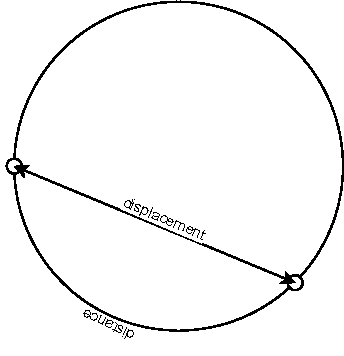
\includegraphics[width=0.4\textwidth]{displacement}
	\caption{Ilustration of distance and displacement.}
\end{figure}

This metric is based on sinusoidal relation between displacement and distance of two point on the circle (as shown in Fig. 3.1). We obtain displacement between edges by computing distance as crown flies between two GPS locations representing their centers. We will mark this distance as \(d_{real}\). Then we will define \(d_{exp}: E^2 \rightarrow \mathbb{R_+}\) which represents the expected displacement of these centers based on distance of shortest path between these two edges. To use the sinusoidal relation to compute the \(d_{exp}\) we would need to know the final length of the tour, which is not known yet and lies somwhere in \(L\). Instead of using one of interval bounds we will choose different approach - we can approximate the relation itself to make it picewise linear. This function is then clearly symetric by \(\frac {l} {2}\) mark, where \(l\) stands for total circumference of the circle. In other words we get a function for which holds \(d_{exp}(x) = d_{exp}(l-x)\). This means we can always count with the shorter distance by circumference and first half of our function. The last step is to exactly count this funtion, we get \(d_{exp}(x)=\frac{2 x} {\pi}\), which means that this function is not dependent on total circumference - that is important fact for continuous resolution of tour roundness.
We define \(d_{exp}\) for edges as well as for individual points around the tour. The expected displacement of two edges will be defined by expected displacement of theirs center points. This metric has one more important feature, it can be customized to different scales of penalization for not completely round tours. This envolves defining the cost function as \par

\(
	p(e_1, e_2) = \begin{cases}
		\frac 
			{\sigma d_{exp}(e_1, e_2)-d_e(e_1, e_2)}
 			{\sigma d_{exp}(e_1, e_2)}
 		& \text{if } d_e(e_1, e_2) < \sigma d_{exp}(e_1, e_2) \\
		0  & \text{otherwise} 
	\end{cases}
\) \par
Where \(d_e\) stands for actual geometric distance between center points.  \(\sigma \in [0, 1]\) parameter is called strictness and in pratcise define what is the same region for the penalisation of the algorithm. For example with sigma close the zero only the really close edges in the same path would be penalized and therefore it is not hard to find even less round solutions with penalization 0. On the other hand, \(\sigma\) set at 1 means penalizing all the edges where is their actual distance smaller than should be by expectations. Finally the total penalization for whole tour \(\pi\), \(p(\pi) = \sum_{i=0}^{N} \sum_{j=0}^{N}\frac{p(e_i, e_j)l(e_i)l(e_j)}{l(\pi)^2}\) this function should approximate the average penalty between two points randomly chosen on the tour. This also means that it gets more accurate when the number of edges and length of the tour increases.


\chapter{Solution proposal}
I have employed two strategies to solve this problem. I examined the outline of solution described in Stroobant\cite{stroobant} and then decided to work with basic unoptimized version from theirs paper. The first task for me was to expand this solution to work with point-to-point tour requests as well as the original version works with cycles. Then we have thought hard about most important parts of the solution and its inner workings. Based on this analysis we proposed tweaked version of the algorithm  which yields slightly worse results but uses significantly less computational resources. There are several further improvements which could be done to bring results of this second method near to the first one. Exact results could be found in the last section of this paper.
The algorithm itself will run in two stages called forward and backward routing. The forward routing part is common for both versions of the algorithm, however the second part is splitted in two section, where both of them describe different strategy to found optimal-like route back.


\section{Forward routing}
First stage, is meant to find all nodes which can serve as "turning point" for the search. These nodes that are acceptable to use as starting point for backward search are called candidates. Base method to find all candidates is rather simple, althoug we can mount many optimalization to it as well as is shown in next sections. For the sake of simplicity let's now consider as candidate every node \(n\) that satisfies the condition \(d(g, n) + l(\pi)\) lies in \(L\). Where \(\pi\) stands for weight-mean-wise optimal path from \(s\) to \(n\). From this specification we can derive the actual procedure to find mentioned candidates.
We are going to run a graph search (most likely the Dijkstra graph search) that starts from starting point defined in the problem instance. This search doesn't search for any goal node but it is hard constrained by length criterium presented earlier. And it uses the weight criterium for edge cost evaluation rather than length of it. There is a fair reason for that. When candidate is found we can immidiately obtain the weight-mean-wise optimal path \(\pi\) mentioned earlier. This path is later used as first leg of our result. The second one is obtained by backward routing.

\section{Backward routing}
I am going to assume we have just one candidate \(t\) linked with proper forward path from earlier. The actual act of selecting from bunch of acceptable candidates is described below. Now we have to find path back from this candidate. This path \(\rho\) starts in \(t\) ends in \(g\), and it has to be true that \(l(\rho) + l(\pi) \in L\). To obtain this back path, we launch yet another graph search from \(t\). This search is aimed toward \(g\), constrained by length and uses mean total cost \(c\), that is introduced above, to order encountered nodes in its open list. Employing total cost in this search has legitimate reason - it ensures that our backward path will respect the need to obtain round and geospatially diverse walk. It makes proportionally to \(\lambda\) and \(\sigma\) harder to revisit the same segment of the road, but it doesn't forbid it completelly, which has positive efect on solvability. And it still respects (except extreme cases) the weight of each edge. From this word specification we can obtain the actual formula to use in backward search. We start with simple mean cost for edge \(e\), \(c(e) = w(e) + \lambda p(e, \pi)\). To get the roundness penalty of selected edge against the whole forward path we will take the roundness penalty formula from previous chapter and limit it to formula \(p(e, \pi) = \frac {2 \lambda} {l_{max}} \sum_{e' \in \pi}{p(e, e') l(e) l(e')}\). This is the last thing needed to complete and launch our search, which if successful yields two paths \(\pi\) and \(\rho\). These paths combined forms our result, path containing all three points \(s, g, t\) with its length in interval \(L\) and mean cost close to optimal. But this is only smaller subproblem. To get close to global optima we have to use another technics mostly to help us select ideal turning points from candidates found in first stage of our algorithm.

\section{Filtering and picking candidates}
From now on I am working with set of candidates obtained in the first stage of the algorithm, all of them fit to serve as a turning point for described backward routing. It would be highly impractical due to overwhelming resource consumption to plan backward path from each of them. Althoug sorting and filtering this set of walks would lead to results which are closest to the optimal one. The most simple approach would be to pick from this set at random but that has obvious impact on result quality. We could easily point the picking mechanism to the candidate set that has much better probability to result in close to optimal set of solutions. One of the options is to sort the candidates by best mean cost of their forward paths. These paths have higher probability to be included in the optimal solution.\par
Another technique is to take into account the geographic location of picked candidates. We can favor picking sets of turning points which are most geospatially diverse. This has several benefits. For one it makes higher the chance to find the optimal solution to the problem instance. The smaller the distance between two turning points the higher the probablity that the optimal paths from the starting point share most of the segments with only small diversion at the end. These close turning point tend to share very similar backward paths also. Therefor even a lot of used turning points in the same bad area won't find optimal solution. And for the second this technique is also benefical for the end user. It naturally yields geospatial diverse sets of solutions. And we know these results are the most attractive for people that use external suggestions for recreational tours as it bring more distinctive choices for the user to choose from.\par
The candidate that is picked as turning point is actually one of the most important factors which have impact on quality of the result as a whole. After this realization we build the first version of algorithm like this - we find the candidate set mentioned earlier, then we filter it with multiple distinctive filters in order to restrict the set to only the most promising nodes. After this filtration we pick some number of random candidates, run the backward routing using them as turning points and sort the results by total mean cost to return the best ones. This strategy of filtering the candidates by multiple criteria beforehand the picking has shown to be pretty effective in combination with previously mentioned methods. Both methods result quality suffer from nodes spaced too densly in the candidate set. You have much greater probability to chose multiple proximate nodes and that have, as I described, negative impact on final dissimilarity in the solution set. It is also much more resource efficient method to filter these candidates before the backward routing than filtering the result set by geospatial diversity afterwards. \par
There are several filters that has turned out to be quite handy for making the resulting tour smoother I will mention and describe some of them in next sections.
\begin{figure}[!tbp]
  \centering
  \subfloat[Removing dead ends]{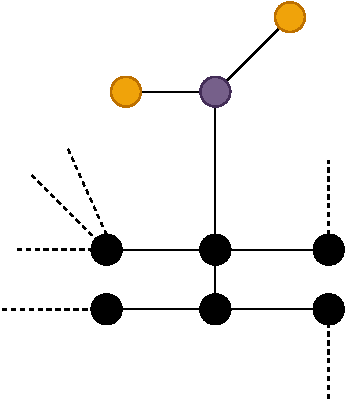
\includegraphics[width=0.4\textwidth]{deadEnds}\label{fig:f1}}
  \hfill
  \subfloat[Node contraction]{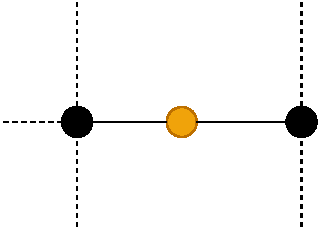
\includegraphics[width=0.4\textwidth]{contracted}\label{fig:f2}}
  \caption{Examples of candidate filtering}
\end{figure}

\subsection{Dead end filter}
The first filter is the one most convenient method to avoid unnecessary returns along the planned tour. The idea behind this filter is to remove all candidates that would, if picked, result in tours that have in the immediate surroundings of the turning point one or more recurring segments. Part of one such tour is displayed in the FIGURE(fill in). Aside from this positive effect, there is also one tradeoff that has to be done. In this problem we take into account the hard constraint on the total length of the tour determined by interval \(L\). By limiting the candidate set you can encounter cases where every tour found is too short and this small segment of return around turning point would add up the length needed in order to get above the lower bound of the interval. \par
The filtering itself run in multiple steps. The first one will remove all the nodes that have only one neighbour in the graph. Each next step will extend this rule to ignore already removed candidates as neighbours. Both steps are pictured in the FIGURE(fill in) where black nodes show candidate nodes, orange ones show nodes removed in the first step and the purple one is the node removed in the next step. Another option to mitigate these tours with returns is to preprocess graph itself before the planner is run. We didn't persue that approach, because althoug we don't want to choose this dead ends as \(t\) we still want this nodes to be available for user to choose them as start node \(s\) or goal node \(g\).

\begin{figure}
	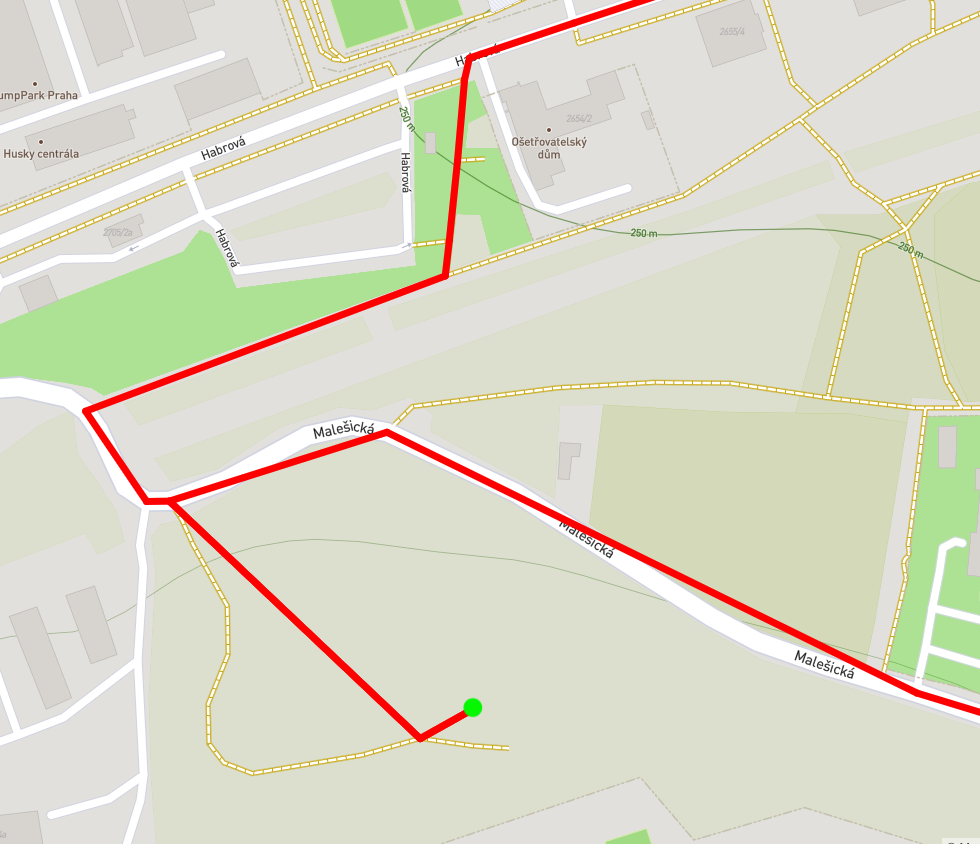
\includegraphics[width=0.7\textwidth]{return.png}
	\caption{Tour with return from turning point located in one of dead ends of the graph}
\end{figure}

\subsection{Contraction node filter} 
Second filter which we proposed and implemented is intended to lower the total number of candidates and higher their mean distance by removing candidates which are surrounded by other acceptable candidates. One of these nodes is pictured in orange in FIGURE(fill in). These nodes have very small impact on quality of the final solution. To explain why, we just need to imagine the case of one simple edge between two points (say \(f\) and \(s\)) with single via node \(v\) in the middle. The via point is of degree 2 and the nodes at the start and end of the edge are of degree 2 or more. Moreover all three nodes are in the candidate set. We choose the point \(v\) as our turning point. It is easy to prove that the path found to this node is (except the very last segment) the same as path found to either \(f\) or \(s\). To revolve around specific case let's think of \(f\). The best path back goes either through \(s\) or \(f\) again. The latter case results in path which is very similar to the one we would get if we chose the the node \(f\) itself, except it has the return around turning point similar to the one described in previous section. The former would result in nice smooth tour. But if this is the case, we would get exactly the same result choosing \(f\) or \(s\) as turning point. Therefor we can neglect that via node with ease. This also holds in more general case when the will be contracted node is of degree more than two with all neighbours in the candidate set. \par
On the top of positive effects on the candidate set mentioned in the opening sentence of this section we get the same tradeoff as in the previous section with this filter. It prunes the solution space from solutions with returns. As mentioned previously this is beneficial to the smoothness of found solutions but also some quite acceptable solutions with returns will be inevitably pruned.

\subsection{Path to distance ratio filter}


\section{Branch and bound algorithm}
The second version of the backward path algorithm does not use any filters and it is very similar to the original version of the algorithm. This version employes different strategy which uses path to the candidate itself instead of single point in order to get the best results. After candidate is picked it gets all nodes on the path from starting node to use every one of them as a turning point \(t\). From each of them is run a version of the backward search described above. As the searches go they are filtered by length criterium and sorted by best cost mean. The best one is then returned as the result for that original candidate.
As I said, this method does not implement filters, but the techniques used for picking the candidates are even more uself than in the first version of the algorithm. Best mean cost path means every segment starting in the \(s\) on that forward path has also the best mean cost. Geospatial diverse candidates are also needed otherwise you could end up iterating many nodes common between close candidates with similar paths multiple times.
We can also restrict the amount of turning points obtained from each candidate. We will simply introduce parameter \(\beta\) which will determine how close we can get to the starting point when getting turning points from the candidate. Specifically we will take into account only nodes \(n\) for which stands \(d(s, n) > \beta\frac {l_{des}-\varepsilon} 2, 1 > \beta > 0\). For values of \(\beta\) closer to zero there is almost no drop in saved resources and quality of the results. Values close to one will drop the whole first half of turning points from the set. 


\chapter{Implementation}
To demonstrate algorithms described above I implemented them as a Java application using Open Source libraries. It is furthermore wrapped as a webservice exposing REST API. Every application can submit parameterized requests for route planning. Best routes are then returned as a response. On top of that I build simple web client in Javascript which can consume the web service and make the process easier for a person. It also provides visualizations and debugging data. All these programs and their architectures are described more thoroughly in the next sections. There is a public version of both client and server code available at the root repository for this thesis.\cite{git}
\begin{figure}[H]
	
\includegraphics[width=0.9\textwidth]{communication}
	\caption{Simple schema of implementation part of this project.}
\end{figure}


\section{Implementation description}
The service and underlying implementation of previously described algorithms is implemented in Java version 8. The whole project is managed in Maven. There are several core dependencies worth mentioning. I implemented the API using Jersey Framework in combination with standart Java Servlet API. This framework makes creating RESTful APIs much easier. It enables using of specific annotations, package specification, custom request filters and more. On top of that Jersey gives out the Jersey Maven plugin. This plugin can deploy the server instance in one command \codeword{mvn clean jetty:run}. After running this command the server is ready to accept the requests to its endpoints via port 8080. \par
\begin{figure}[H]
	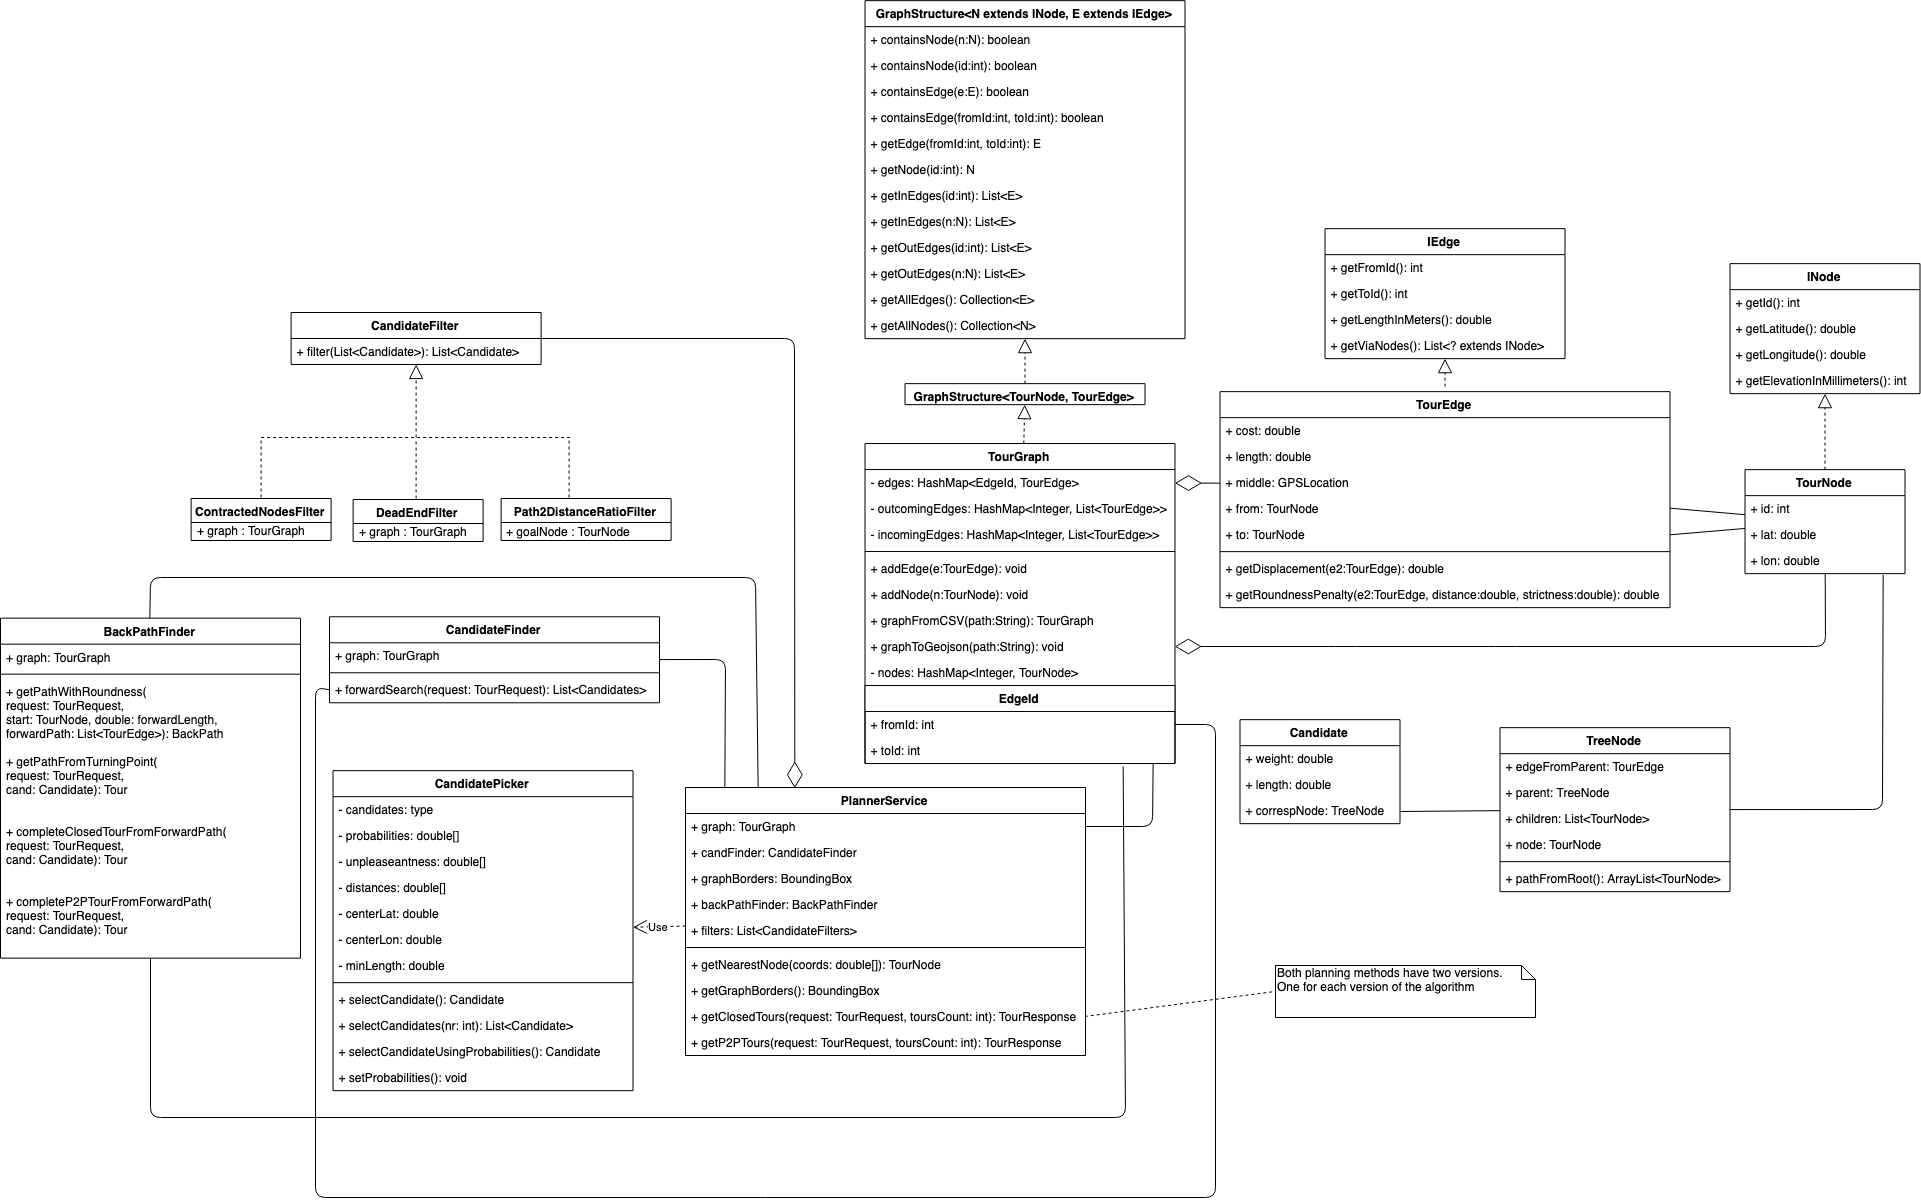
\includegraphics[width=0.8\textwidth]{service.png}
	\caption{Service objects structure}
\end{figure}
Created API and service infrastructure was linked to the \codeword{PlannerService} object that could be seen in the figure. This static object manages all backend logic. At the start of the service it loads graph, creates index over all nodes, create complementary objects as are \codeword{CandidateFinder} or \codeword{BackpathFinder} and more. After this boot up phase it exposes method which corespond to web service endpoints and supply the planning functionality over the API. Every planning request has three stages of execution which are described below. For the representation of graph and its individual features I chose to implement interfaces from \codeword{base-structures} library provided to me by Umotional company. Its interfaces which I used (more specifically \codeword{INode}, \codeword{IEdge} and \codeword{GraphStructure}) encapsulates basic methods on the objects in order to make it absolutely convenient to work with them. Implementations of all these interfaces which I used are available in \codeword{model} package. Second big motivation for this approach was the ability of other libraries to work with these interfaces. \par
To implement forward and backward searches themselves I chosed to use yet another open source library from Umotional company. It is \codeword{core-planning-algorithms}. The library provides functional framework to implement almost any graph search algorithm. It creates higher level of abstraction with help of several general interfaces that encapsulates the basic actors or methods present in every graph search. Everyone can than create their own implementation of these interfaces. Moreover it already provides implementation of basic well-known algorithms as is for example Dijkstra or A*. I used this implementation of Dijkstra, in combinantion with custom made classes pictured in the picture below. 

\begin{figure}[H]
	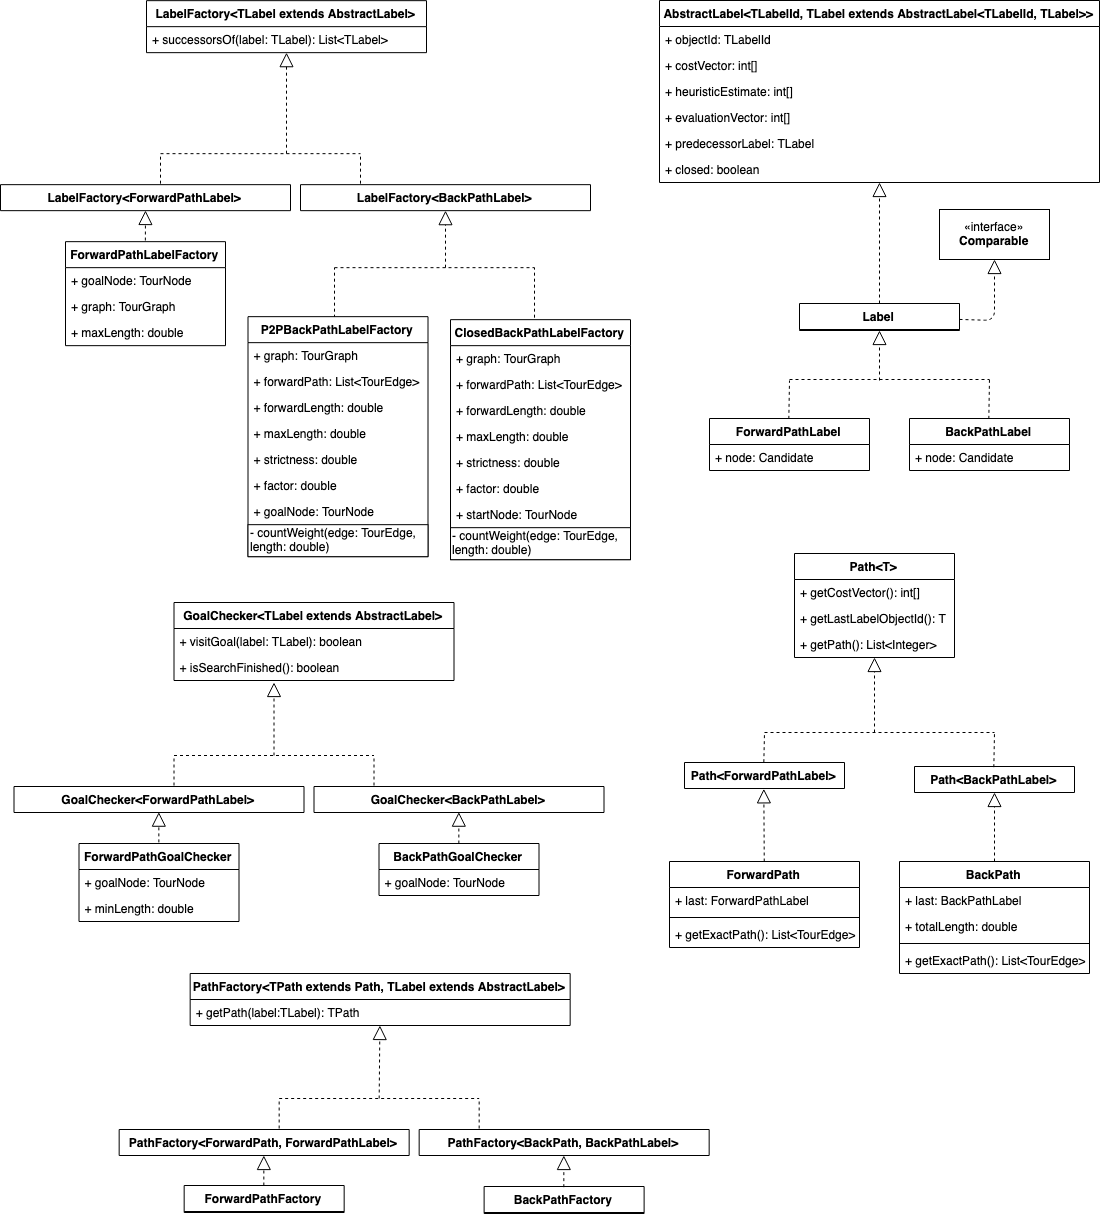
\includegraphics[width=0.6\textwidth]{search.png}
	\caption{Structure of objects used in searches}
\end{figure}



\section{Communication}
As I mentioned before the protocol used in communication with server is REST. There are several methods that can be invoked via web call to relevant endpoint. Each method accepts data in form of querry parameters that are passed on to the service implementation as arguments.

\begin{figure}[H]
	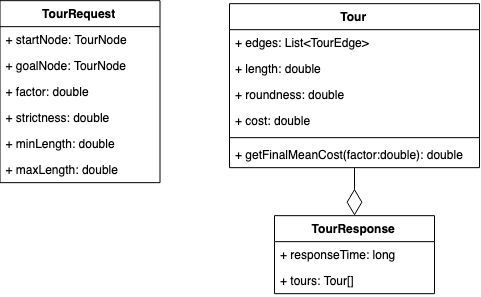
\includegraphics[width=0.7\textwidth]{api.png}
	\caption{Planning request and response objects}
\end{figure}

\subsection{Closed Tours endpoint}

\subsection{P2P Tours endpoint}

\subsection{Nearest Node endpoint}
The core functionality of the service i.e. the planning of the tours described above is designed to accept just a node id as a part of the TourRequest. Although this makes the communication easier from development side of view it is not very convenient for the end user. Therefor this endpoint is available - to translate pair of coordinates into the id of the nearest node in the graph. The most obvious use case for this endpoint which is also used in my client implementation is to let the user click at some point in the map and obtain the nearest node id to use in the actual request. \par
The inner working of this method is provided by KDTree object. This static object is created together with the service and filled up with every node in used graph. We choose object dimension in the size of two as our coordinates has two components also. This allow us to use the basic great circle distance of two points as the resolver function when searching through the KDTree. In the end this approach greatly outspeed sorting or filtering nodes in simple list, but with slightly worse space complexity.

\subsection{Graph Borders endpoint}
This is just a simple enpoint that serves to either visualize the graph borders in the client appliccation or to restrict the requests entered by user to fit currentlly loaded graph.  It returns the greater bouunding box of the graph in GeoJson format. 


\section{Client}

\chapter{Results}
\section{Performance}
\section{Roundness}
\section{Usability}



\chapter{Conclusion}

\begin{thebibliography}{1}
	\bibitem{stroobant}Stroobant, P., Audenaert, P., Colle, D., \& Pickavet, M. (2018). \emph{Generating constrained length personalized bicycle tours.} 4OR, 16(4), 411–439. \url{https://doi.org/10.1007/s10288-018-0371-9} 
	\bibitem{karp}Karp, R. M. (1978). \emph{A characterization of the minimum cycle mean in a digraph.} Discrete Mathematics, 23(3), 309–311. \url{https://doi.org/10.1016/0012-365x(78)90011-0} 
	\bibitem{oatsp}Maervoet, J., Brackman, P., Verbeeck, K., De Causmaecker, P., \& Vanden Berghe, G. (2013). \emph{Tour Suggestion for Outdoor Activities}. In Web and Wireless Geographical Information Systems (s. 54–63). Springer Berlin Heidelberg. \url{https://doi.org/10.1007/978-3-642-37087-8_5} 
	\bibitem{jogging}Gemsa, A., Pajor, T., Wagner, D., \& Zündorf, T. (2013). \emph{Efficient Computation of Jogging Routes.} In Experimental Algorithms (s. 272–283). Springer Berlin Heidelberg. \url{https://doi.org/10.1007/978-3-642-38527-8_25} 
	\bibitem{juraska} Juraska, J., Nykl J. (2016). \emph{Multi-criteria Route Planning with Emphasis on Geospatial Result Diversity} \url{https://www.semanticscholar.org/paper/Multi-criteria-Route-Planning-with-Emphasis-on-Juraska-Nykl/96165d905691de3b8e9b0af8b83fc2e68941b59c}
	\bibitem{git} Matocha, M., \emph{bp}, (2019), GitHub repository, \url{https://github.com/Shade254/bp}
\end{thebibliography}
\end{document}